\documentclass[12pt, b4paper]{article}
\usepackage[margin=2cm]{geometry}

\usepackage{graphicx} % Required for including images
\usepackage{animate}
\usepackage{caption}
\usepackage{subcaption}

\usepackage{booktabs} % Required for better horizontal rules in tables

\usepackage{listings} % Required for insertion of code
\lstset{
  basicstyle=\scriptsize\tt,
}

\usepackage{enumerate} % To modify the enumerate environment
\usepackage{enumitem} % to contorl the numbering behavior

\usepackage{verbatim}

\title{Security of Payment Project: using machine learning models to help adjudication applicants be better prepared}

\author{
\begin{tabular}{ c c }
    Shengyang Sun & 1418346 \\
 \end{tabular}
 }


\begin{document}

\maketitle

\tableofcontents

\newpage

%-----------------------------------------------------------------------------------------------------------------------------------------

  \section{Introduction}
    \subsection{Background}
    SOP, or security of payment, is an Act to provide entitlements to progress payments for persons who carry out construction work or who supply related goods and services under construction contracts. 

    \subsection{Dataset}
    The dataset contains the application information for period between May 2021 to June 2022. We categorized the attributes based on the chronological order, i.e. whether they happen before, at, or after the determination of adjudication. 'Before' attributes contains key date, description of work, procedural documents potentially required during the application, monetary amount, and company information pertaining to both the claimant and the respondent and are basically used as candidate predictors for our main response variable used in regression model: Adjudicate ratio, 'At' attributes (or we call 'FACT') are information about the actual adjudication determination and variables we try to predict. 'After' attributes are mainly the breakdown of adjudicator fees between claimant and respondent, ANA and adjudicator and will not be of much interest to us with regard to the scope of our analysis.

    \subsection{Research Question and Target Audience}
    Our target audience would be the potential users of the SOP service, we strive to answer the following question for them:
    \begin{quote}
        \textit{For a potential user of the SOP service, given its before application condition, should it use the SOP service?}
    \end{quote}
    We'll address this question by considering 3 criteria:
    \begin{enumerate}
        \item Is potential claimant's work provided covered under SOP?
        \item What is the potential claimant’s standing among all the previous applicants?
        \item Given the potential claimant's prior-to-application situation, what is his expected 'Adjudicate ratio' defined as: 
          $$Adjudicate\ ratio = \frac{Adjudicated amount}{Claimed amount}$$
    \end{enumerate} 
    Each of the questions will be answered by applying knowledge of NLP, visualisation, and supervised machine learning model respectively. \\ 
    Another potential audience of our research is Victorian government because we might expose some of SOP act's merit during our research which will encourage more people to use adjudication service instead of taking to the legal path, thus saving public resource.

%-----------------------------------------------------------------------------------------------------------------------------------------

  \section{Data Wrangling}
    \subsection{Data Cleansing}
    Like every raw, unprocessed dataset, our adjudication dataset comes with numerous issues for us to address. Different categories of problematic data are briefly discussed below, and some representative cases are listed. For a full list of the preprocessing that we have done to the dataset to prepare it for a smooth data analysis, please refer to our source code.
    \begin{enumerate}
      \item Missing data: these are the data that are simply missing. 
        \begin{itemize}
          \item Cases that are 'not \textbf{yet} determined' contains no information about adjudication determination and are thus discarded.
          \item 'Respondent advisers' has 42 cases of 'Not Known' which essentially are missing values. We imputed randomly chosen values based on the distribution of all the non-null values. 
        \end{itemize}
      \item Logically or legally contradictory data: 
        \begin{itemize}
          \item Cases that are determined but has value in the column 'Reason not determined' are logically contradictory. So we set the reasons to null.
          \item Cases that are applied under section 18(1)(b) (which is the case that the respondent does not provide payment schedule) but the 'Payment schedule provided' column has value 'Yes'. We set them to 'No'.
        \end{itemize}
      \item Highly skewed variable and outliers.
        \begin{itemize}
          \item Outliers can have a huge leverage on the outcome of a regression model thus must be dealt with. In our dataset, 'Claimed amount' is highly skewed with an outlier of magnitude 34 million while majority of the data has value only under one million. This situation is ameliorated by log transformation as evidenced by the almost normal distribution after the transformation. (Figure~\ref{fig:BBlogTrans})
      \begin{figure}
        \centering
        \begin{subfigure}{.5\textwidth}
          \centering
          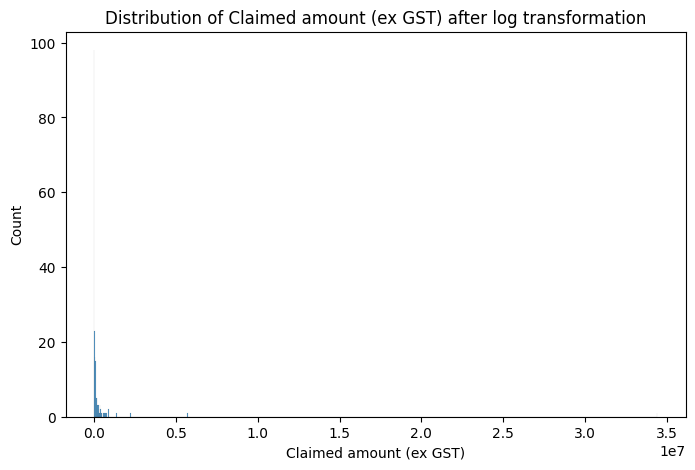
\includegraphics[width=.8\linewidth]{plots/distClaimAmountBeforeLog.png}
          \caption{Claimed Amount Before Log Transformation}
        \end{subfigure}
        \begin{subfigure}{.5\textwidth}
          \centering
          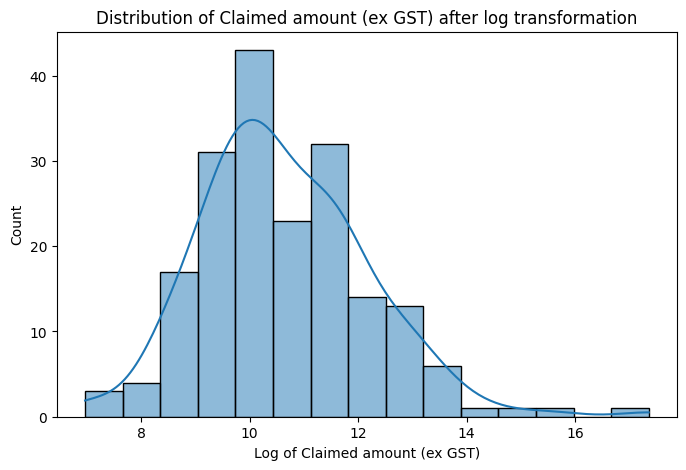
\includegraphics[width=.8\linewidth]{plots/distClaimAmountAfterLog.png}
          \caption{Claimed Amount After Log Transformation}
        \end{subfigure}
      \caption{Comparison of distribution before and after the log transformation}
      \label{fig:BBlogTrans}
      \end{figure}
            
        \end{itemize}
      \item Wrong data
        \begin{itemize}
          \item 'Determination release date' has some rows with value 00-Jan-1900 which is the starting value of Excel's time which basically means null value. 
        \end{itemize}
      \item Perfectly correlated or not informative attributes: 
        \begin{itemize}
          \item The information of whether the respondent has provided a payment schedule is implicitly embedded inside 'Section of Act application made under'. For example, if an application is made under s.18(1)(b), that means the respondent has not provided any payment schedule which means we could safely remove the column 'Payment schedule provided' without losing any information.
        \end{itemize}
    \subsection{Extract meaning from text}
    After we finished all the cleansing, we assign each column to an appropriate data type before the last step of our data preprocessing: extracting meaning from the two string type variables:  
      \begin{itemize}
        \item 'Description of project and contract works': \\
          This attribute is a small string of texts that is humanly readable but is very hard to incorporate into the data analysis, especially fitting into a regression model. What we do is applying some basic NLP techniques to transform them into a word count vector and performed a classification using K-mean with k=7. The reason we chose 7 is that there are 7 categories of construction that is covered under the SOP act. K-mean is a preferred classification method here because is an unsupervised ML technique and thus does not require a previously labeled data.
        \item 'Project postcode': \\
          Postcode has more than 130 categories while our data only contains more than 300 observations. We reduced the granularity of postcode by assigning postcode to LGA, which reduces the number of categories to 5. 
      \end{itemize}

    \end{enumerate}

    \subsection{Exploratory Data analysis}
    In this section we explored the dataset with some EDA techniques to give the potential applicant a high-level picture of the SOP act. 
      \subsubsection{Descriptive statistics}
      Some high-level overview of the SOP act.
        \begin{itemize}
          \item Out of all the applications during the dataset period, 61.89\% of them are determined. Reasons for cases not determined are withdrawal, settlement between parties and time-out.
          \item Although the SOP act requires the adjudicator to determine an application within 10 business days (s.22(4)(a) in SOP act) or 15 extra days if the respondent seeks to extend it under s.22(4)(b), you should not be too surprised if that takes longer than 10 days because that happens more than half of the time. If the respondent has applied for extension, you should expect the determination to arrive around 15 days with rare extreme case where it took more than 30 days to arrive at the determination. (Figure~\ref{fig:daysAccepComp}) 
            \begin{figure}
              \begin{center}
                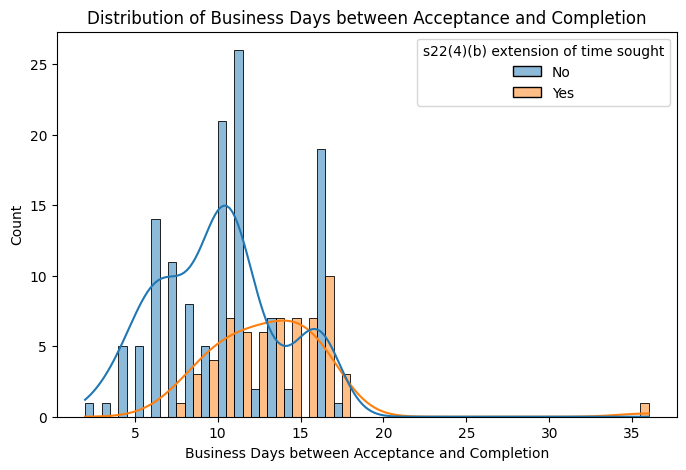
\includegraphics[width=0.6\textwidth]{plots/daysAccepComp.png}
              \end{center}
              \caption{Distribution of Business Days between Acceptance and Completion}
              \label{fig:daysAccepComp}
            \end{figure}
        \end{itemize} 

      \subsubsection{Pairwise Relationship}
      We plotted a heatmap for all the continuous variables in the dataset (Figure~\ref{fig:corrAll}). Here are just a few of the interesting findings: 
      \begin{itemize}
        \item Adjudicator fee is proportional to claimed amount but not in a strictly linear fashion that means it has some sort of soft cap which is evidenced by a higher correlation of 0.73 between 'adjudicator fee' and 'log claimed amount' than that of 0.4 between 'adjudicator fee' and 'claimed amount'.
        \item The more justified your application is (as shown by a high adjudicate ratio), the less you need to pay for the adjudicator fee. This is evidenced by a -0.76 correlation between 'Adjudicate ratio' and 'Adjudicator's fee payable by claimant'.
        \item The longer it takes to determine the adjudication, the higher adjudicator fee one need to pay. This is evidenced by a 0.39 correlation between 'Business day between application and acceptance' and 'Adjudicator fee'.
      \end{itemize}

      \begin{figure}
        \begin{center}
          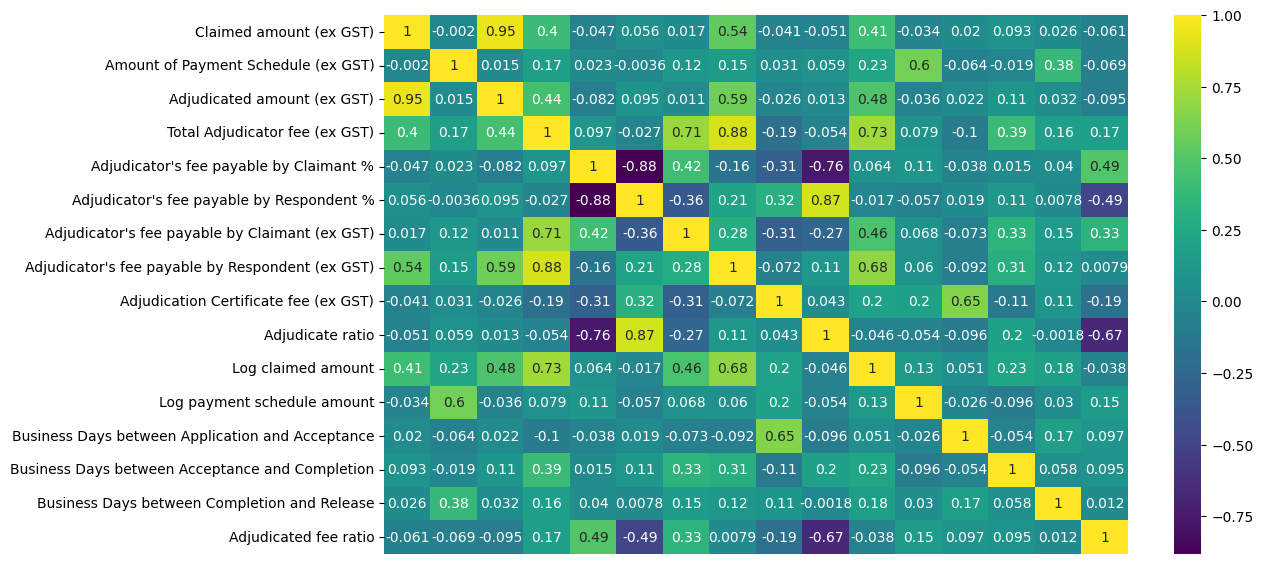
\includegraphics[width=\textwidth]{plots/corr_all.png}
        \end{center}
        \caption{Pairwise Relationship within continuous variables}
        \label{fig:corrAll}
      \end{figure}
     
     Another thing a potential claimant might worry about is that is he going to be discriminated because of the magnitude of his claimed amount. The answer is a clear no as evidenced by Figure~\ref{fig:AdjRatioToLogClaimAmount} where we can see the there is no distinguishable pattern with the change of claimed amount.
     \begin{figure}
      \begin{center}
        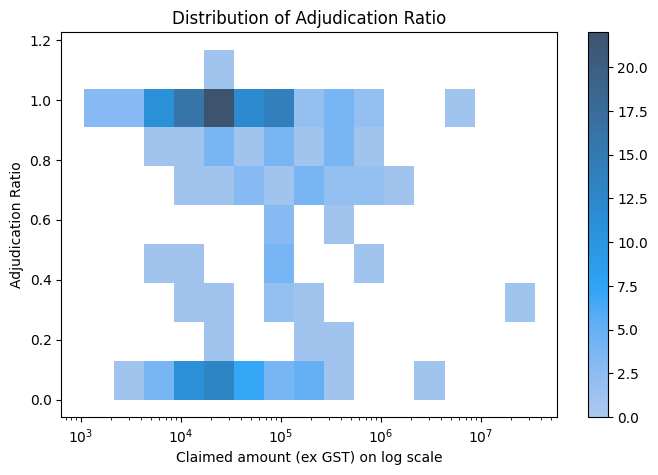
\includegraphics[width=0.6\textwidth]{plots/AdjRatioToLogClaimAmount.png}
      \end{center}
      \caption{Histogram of Adjudicate Ratio and Log Claimed amount}
      \label{fig:AdjRatioToLogClaimAmount}
     \end{figure}
     

      \subsubsection{Using OpenAI API to inform claimant whether his construction work is covered under SOP act}
      The legal document dictates seven categories of construction works that are covered under SOP act and three that are not. We prompted the user to input the type of construction work that he has provided and feed this information along with the covered/not covered categories into a OpenAI language model to ask it to classify whether the work performed is covered or not. You can find a working example of it in Figure~\ref{fig:OpenAI}. Although for SOP, the definition of covered work is quite simple and people can just refer to it without any legal counsel. This technique can definitely be generalized to more complex legal definitions.
      \begin{figure}
        \begin{center}
          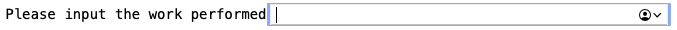
\includegraphics[width=0.6\textwidth]{NLPimage/img1.png}
          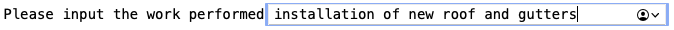
\includegraphics[width=0.6\textwidth]{NLPimage/img2.png}
          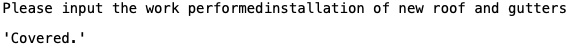
\includegraphics[width=0.6\textwidth]{NLPimage/img3.png}
          
\includegraphics[width=0.6\textwidth]{NLPimage/img4.png}
          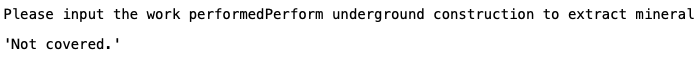
\includegraphics[width=0.6\textwidth]{NLPimage/img5.png}
        \end{center}
        \caption{Working example of work type filtering}
        \label{fig:OpenAI}
      \end{figure}
      
%-----------------------------------------------------------------------------------------------------------------------------------------

  \section{Feature Selection}
  For feature selection, we performed Pearson's correlation between response and continuous variables and Mutual Information categorical ones. This is cross validated with the visualisation analysis. Because we don't have domain knowledge in either legal or construction area, the computed values are compared relative to each other instead of having an absolute threshold. 
  \subsection{Pearson's Correlation}
  Claimed amount suffers from some serious outlier issues and that's why we log transformed it to bring it back to a close to normal distribution. The effect can be clearly seen in the correlation matrix. Without this adjustment, one would wrongly believe that there's almost no relationship between claimed amount and response when in fact they are highly correlated. (Figure~\ref{fig:correlations})
  \begin{figure}
    \begin{center}
      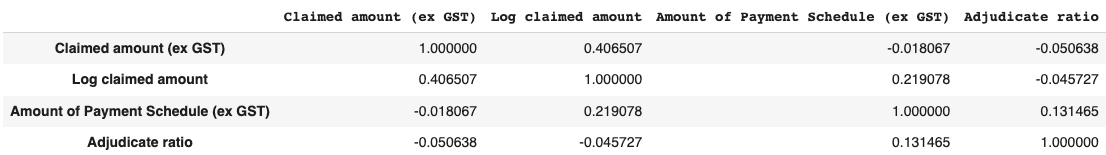
\includegraphics[width=0.95\textwidth]{plots/correlations.png}
    \end{center}
    \caption{Correlation matrix between response and continuous variables}
    \label{fig:correlations}
  \end{figure}

  \subsection{Mutual Information}
  Mutual information is calculated between response variable and 'BEFORE' categorical variables to discern those that possibly has a predicting power over response. 
  \verbatiminput{code\_output/MI\_response.txt}

We can see that relatively, 'Section under Act application made under', 'Claimant adviser', 'Business Type/Activity (Respondent)' have higher MI values. But in absolute term, their values are pretty low ranging from 0.07 to 0.09, and thus we'll not rule out any candidate variables for now and do some significance testing during model fitting stage and hope that the results will corroborate. 

%-----------------------------------------------------------------------------------------------------------------------------------------

  \section{Model Fitting}
  \subsection{The purpose of the model is two-fold}
  \begin{itemize}
    \item To give potential claimant a general idea of how much he is expected to receive (as a percentage of his claimed amount) through the SOP service.
    \item To inform potential claimant which factors could have a significant influence on the outcome of the adjudication result so that claimant can be more prepared.
  \end{itemize}

  \subsection{Justification of Model Choice}
  We choose to use Beta regression to fit our data because our response variable: the 'Adjudicate ratio', is a percentage value and is bounded by (0, 1). Also percentage value tends to have heteroskedasticity and skewness issues, which means their variance is higher in the middle and lower at the two extremes, and the distribution is not normally distributed. Both of these characteristics is clearly visible in the histogram of the response variable (Figure~\ref{fig:responseDist}). Beta distribution is naturally heteroskedastic and can easily accommodate asymmetries. 
  \begin{figure}
    \begin{center}
      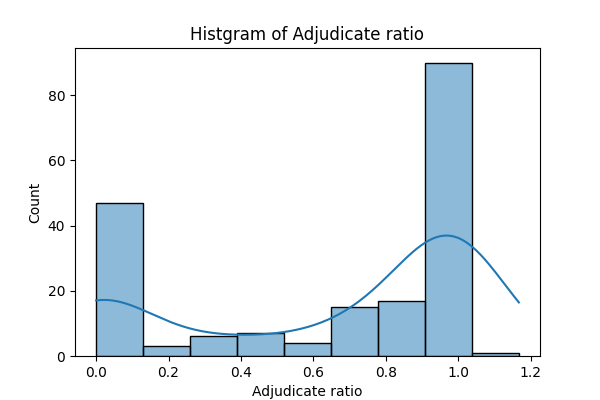
\includegraphics[width=0.6\textwidth]{plots/AdjudicateRatioHist.png}
    \end{center}
    \caption{Histogram of Adjudicate Ratio}
    \label{fig:responseDist}
  \end{figure}

  \subsection{The procedure of the model fitting}
  \begin{itemize}
    \item randomly split dataset into train and test, the ratio is set at 90:10 because we want to have as much data in the train set as possible to avoid structural zero issue. 
    \item Include every candidate predictors into the model.
    \item Filter out any insignificant predictors based on Wald test using 95\% as critical value.
    \item Try to further remove variables and test whether they have as good fitness as the larger model using Likelihood Ratio Test to try to achieve an even more parsimonious model.
    \item Two link function, i.e. logit link and loglog link, are compared. Theoretically, loglog link should perform better with a dataset skewed toward the 1 side (large extreme value), but the two models have almost the same AIC. So we just arbitragely chose a more parsimonious model which uses loglog link. 
    \item The model is used to predict the outcome of the test set.
  \end{itemize}
  \subsection{Final model}
  Our final model is as follows (notice some categories are discarded due to structural zero issue) (Listing~\ref{finalModel}): 
  \lstinputlisting[float=h, frame=tb, caption={R output}, label=finalModel]{code\_output/final\_model.txt}

  \subsection{Interpretation of the Model} 
  The final model turns out to be parsimonious, intuitive, informative all at the same time, which is super great! 
  \begin{itemize}
    \item The coefficient of 0.5318 means comparing to applications applied under s.18(1)(a)(i) (where the respondent provided payment schedule), those applied under s.18(1)(b) (where the respondent failed to provide payment schedule) has $e^{0.5318} - 1 = 70.2\% $ higher log(Adjudicate ratio). 
    \item The coefficient of -0.6286 means comparing to applicants who have a preparer to help with the application, those do not have any adviser has a $1 - e^{-0.6286} = 46.67\%$ lower log(Adjudicate ratio).
    \item The coefficient of -0.1613 and its insignificance means the effect of having a solicitor helping you with application is as good as having a preparer.
    \item In summary, a claimant is in a more advantageous position if the respondent does not provide a payment schedule, and he has some professional to help preparing with the application.
  \end{itemize}

  \subsection{Performance}
  Overall, we don't expect our model to behave greatly in terms of predicting power as suggested by the low correlation and mutual information calculated in the feature selection section. This is evidenced by a low 'Pseudo R-squared' value of 0.1865. Besides, the final model only have 2 x 3 = 6 levels in total which means there can only be 6 possible predictions. Since most of the adjudicate ratio is 100\%, we are bound to have larger over-estimation problems for those data points with a low adjudicate ratio and milder under-estimation problems for those data points with a adjudicate ratio close to 1. This is evidenced by the raw residual plot (Figure~\ref{fig:rawResidualOnTest}). 
  \begin{figure}
    \begin{center}
      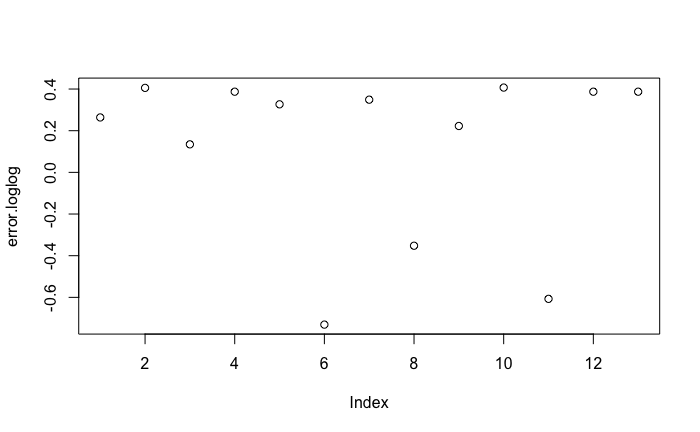
\includegraphics[width=0.6\textwidth]{plots/rawResidualOnTest.png}
    \end{center}
    \caption{Raw residual of prediction on the test set}
    \label{fig:rawResidualOnTest}
  \end{figure}
  

  \section{Limitation and Future Improvement}
  \subsection{Preprocessing}
  The logical relationship between varialbes is very intricate and intertwined which makes the ordering of our preprocessing very vulnerable. A single switch of ordering between steps could render following steps unfunctional.  
  This signals that our preprocessing is not very robust and is too specific to our dataset to generalize to other datasets.  
  On the other hand, the nature of our preprocessing is highly accurate which satisfied both legal requirement and logical constraints instead of just dealing with missing values and mis-inputs. 
  So it's really hard to strike a balance between robustness and accuracy
  \subsection{Feature Selection}
  Some domain knowledge in legal and construction will help us to better filter the features.
  \subsection{Model Fitting}
  If we have the time, we could incorporate adjudicator fee into our model to give the claimant a more accurate estimate of the amount he is going to receive.  
  We could also reverse engineering to try to deduce how the adjudicator fee and certificate fee are calculated.
  Limited by the small data size, there would be a lot of structural zeroes if we try to include interaction terms in the model. Some of the variable pairs definitely have the potential of being predictive such as claimant's business activity:respondent's business activity, and region:type of construction work. With a larger dataset, model with higher order terms could be achievable.


 % \section{section2}
 %   \begin{figure}
 %     \begin{center}
 %       \includegraphics[width=0.6\textwidth]{figures/}
 %     \end{center}
 %     \caption{}
 %     \label{fig:}
 %   \end{figure}
 %   
 %   \begin{table}
 %     \caption{}
 %     \label{tab:}
 %     \begin{center}
 %       \begin{tabular}[c]{l|l}
 %         \hline
 %         \multicolumn{0}{c|}{\textbf{}} & 
 %         \multicolumn{1}{c}{\textbf{}} \\
 %         \hline
 %         a & b \\
 %         c & d \\
 %         
 %         \hline
 %       \end{tabular}
 %     \end{center}
 %   \end{table}    

\end{document}
